\chapter{Design}

\section{Architecture} \label{arch-design}

The designed architecture of the project can be observed in the figure \ref{fig:arch}. There are three data sources connected to Grafana through an extended version of the official SimpleJSON data source plugin:

\begin{itemize}
	\item RapidMiner Server
	\item JSON backend
	\item Python data source
\end{itemize}

Each data source accesses the data it provides to Grafana in different ways; through an outside service, from a database or from memory.

\begin{figure}[h]
	\centering
	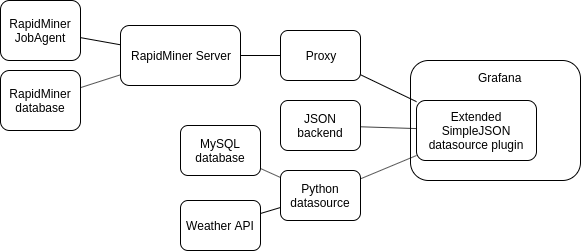
\includegraphics[width=150mm, keepaspectratio]{figures/architecture.png}
	\caption{Architecture diagram}
	\label{fig:arch}
\end{figure}

%---
\section{Components}
%---

In this section, each component's design is presented, focusing on their responsibilities.

%---
\subsection{Extended SimpleJSON datasource plugin} \label{simplejson-design}
%---

Grafana uses data source plugins to connect to different data storage backends. These components usually poll their backends, sending query requests to acquire the recorded information. Each data source plugin exposes a Grafana specific interface which allows Grafana to communicate with each data source plugin the same way.

% https://github.com/grafana/simple-json-datasource
The SimpleJSON datasource is made by the Grafana team and is available on GitHub (insert reference HERE).

It has two main purposes. One is to act as an example implementation to make writing custom data source plugins easier for the community. The other is to enable Grafana to read data from services that expose data in JSON format (which is widely popular thorough the industry).

For this thesis project, the latter role seems to be more important, as it is possible to create a tool that receives data from different kind of formats and translates them into JSON. This way, we can send the transformed data to Grafana, which as a result, would be able to display the collected data that originally came from various sources in one place .

Hence, instead of designing a data source plugin for Grafana from scratch, I chose to customize this already available component to dodge many caveats of developing an own plugin for a complex system.

% https://github.com/grafana/simple-json-datasource/blob/master/README.md
The SimpleJSON data source plugin requires its backend to implement the following endpoints:

\begin{itemize}
	\item \emph{/} - This endpoint is used for testing the connection between Grafana and the data backend. If everything is in order on the side of the backend, this endpoint should return a HTTP 200 response.
	\item \emph{/search} - This endpoint is used for finding the available metric options. For example the names of different time-series.
	\item \emph{/query} - This endpoints is used to acquire the actual metrics data from the backend.
	\item \emph{/annotations} - This endpoint is used to return objects called annotations that are additional information attached to metrics data. In the context of this project, we do not use this feature, however, it is needed for the data source plugin to run without errors.
\end{itemize}

In order to introduce additional interactivity capabilities, when integrating the RapidMiner web service, the SimpleJSON data source plugin needs to be extended. Since it is possible for a RapidMiner web service to accept parameters, which can filter the result, it would be useful to be able to acquire these available exposed parameters, so we can make more accurate metric queries with Grafana.

This means that the plugin has to be able to send another type of request to the backend, which in return would respond with the list of the accessible parameters:

\begin{itemize}
	\item \emph{/parameters} - This endpoint is used for acquiring the available query parameters exposed by the backend.
\end{itemize}

During operation, this data source plugin will periodically poll its connected data sources for data, sending HTTP requests to the above described endpoints. The time-interval between the polls depends on the settings in Grafana.

%---
\subsection{Proxy (Gateway)} \label{proxy-design}
%---

The main responsibility of this component is to translate between the RapidMiner web service, which the RapidMiner Server exposes and the SimpleJSON data source plugin. The problem is that RapidMiner Server makes its result available in JSON, but in another format, than the SimpleJSON data source plugin accepts.

To accomplish that this proxy component could communicate with Grafana, it must implement the endpoints required by the SimpleJSON plugin. These were explained in the section \ref{simplejson-design} describing the plugin.

So the gateway component should be able to handle HTTP requests from SimpleJSON as well as forwarding them to RapidMiner after the translation. For this reason, it must be a constantly available service.

There are some RapidMiner web service specific considerations which need to be taken into account while designing the gateway component. We have to define the actions made by the proxy towards the RapidMiner Server in an abstract way, in order to properly implement the component.

%---
\subsubsection{Searching the targets}
%---

In order for Grafana to be able to make queries to request data, it needs to know where this data can come from, what is the address of the service that exposes the recorded information. For that, Grafana (and indirectly the SimpleJSON data source plugin) first asks for the available targets of the given data source backend. As it was mentioned in section \ref{simplejson-design}, SimpleJSON uses the \texttt{/search} endpoint for acquiring this information.

In our case, the Proxy component connects to RapidMiner Server which exposes its data providing processes through web services. Thus, when accepting requests on the \texttt{/search} endpoint the gateway should return with the names of the available RapidMiner web services in a format that the data source plugin accepts. For that, it must send a request to the RapidMiner Server, asking for these names each time, so it is ensured that the information is always up-to-date. This is crucial, as the name of the RapidMiner web service determines the address where the gateway has to send the query requests later.

%---
\subsubsection{Acquiring the parameters}
%---

To enable the customization of the queries, the Proxy's \texttt{/parameters} endpoint should return the parameters exposed by a given web services. This information also falls in the category that should not be cached, as the possession of false knowledge can lead to failed queries that ends up in no data displayed in Grafana.

%---
\subsubsection{Querying the data}
%---
After we have the name of the web service and its available parameters, we can finally request the actual data. To accomplish that,  Grafaba sends a request to the \texttt{/query} endpoint of the Gateway component. Grafana can handle data in two formats: time series, and table. This means that the Proxy component should be able to convert the acquired data from its backend into one of these formats.

%---
\subsection{JSON backend}
%---
% https://github.com/bergquist/fake-simple-json-datasource
This component is a example backend implementation for the SimpleJSON data source plugin. It serves as a base for creating other backends for the data source plugin. It also further expresses the general usability of the SimpleJSON plugin.

As this component can work with the SimpleJSON data source plugin out-of-the-box, I used it during the thesis project mainly for testing purposes. For example to check if the connection is still healthy between the components, or to inspect the specific data formats which are sent to or received from the SimpleJSON plugin.

%---
\subsection{Python data source}
%---

Although Grafana has multiple built-in plugins to communicate with databases, there exists some use-cases, when having a custom component between the data source and the visualization tool is feasible.

With an additional component in the middle, we have extra control over the data which travels from the data storage backend (in our case, MySQL) to the visualization platform. This means that we do not have to rely solely on the capabilities of the database, which can lead to simpler queries and smaller communication overhead with the database.

Having a custom middleware also makes it possible to implement the business logic in a separate component and only display business-relevant information with the visualization tool.

It also enables us to aggregate information from different backends and provide only one kind of interface towards the visualization which can result in better maintainability. For example in our case, the Weather API component acts as a second backend.

Similarly as the Proxy component, the Python data source also needs to have those endpoints which are required by the SimpleJSON data source plugin, so this part is analogous to that in the Proxy. The effects of invoking them are slightly different than in case of the Gateway, because this Python source uses two components as backends, the 'external' API service and a separate database as described in section \ref{case-study-python-source}. So in order to get the requested data, the Python data source has to turn to both of its backends. This means, that the Python data source has to possess more sophisticated communication capabilities. It needs to be able to handle requests from Grafana, send them back, make connections to the database and query its contents and to send requests to the 'external' API service and accept the results from it.

%---
\subsection{Weather API}
%---

As it was already described in section \ref{case-study-python-source} describing the sample use-case, I implemented a simple service, that can return the all-time (calculated in a heuristic way, as it was already mentioned) maximum and minimum temperatures measured in New York for a given day of the year.

This component represents the previously mentioned external service. Its responsibility is to expose a service that can be utilized by other softwares in order to acquire additional business-relevant information.

It is worth to mention, that there are already several publicly available APIs that can be used to retrieve weather related data. For example, the API services of OpenWeatherMap or AccuWeather. However, these services are usually not free or only offer a free trial version which lasts just a couple a days long. This is why I decided to make an own API service that can be used during the whole time of preparing the thesis project.


% https://openweathermap.org/api
% https://developer.accuweather.com/
\begin{center}
	--- TODO ---
	references for the weather apis
\end{center}

%---
\subsection{MySQL database}
%---

In section \ref{case-study-python-source}, it was stated, that one the backends used by the Python data source is a separate database. This database stores the data of the measured daily maximum and minimum temperatures in New York throughout a couple of years.

%\begin{itemize}
%	\item why do we need a gateway
%	\item how can we access data from RapidMiner WebService
%	\item why is it good to have a python compoment between Grafana and MySQL
%	\begin{itemize}
%		\item we can customize it better, what we see from the database
%		\item can implement business logic, only see business-relevant projections, granularity of the data
%		\item can aggregate data from different backends
%		\item can aggregate data with outsider APIs (POC implementation for this use-case)
%	\end{itemize}
%\end{itemize}


%\begin{itemize}
%	\item Grafana
%	\item proxy/gateway
%	\item python-datasource
%	\begin{itemize}
%		\item python-datasource
%		\item mysql
%		\item weather-api
%	\end{itemize}
%	\item RapidMiner stack
%	\begin{itemize}
%		\item rapidminer-server
%		\item job-agent
%		\item database
%	\end{itemize}
%	\item Grafana datasource plugin (extended API - parameters)
%	\begin{itemize}
%		\item extended API for asking for available parameters
%		\item extended GUI, that dynamically lists available parameters (specify SOURCE!!!!!!!)
%	\end{itemize}
%	\item Grafana extended panel plugin
%\end{itemize}